%
% paradox.tex
%
% (c) 2019 Prof Dr Andreas Müller, Hochschule Rapperswil
%
\section{Haar-Approximation
\label{haar:approximation}}
\rhead{Haar-Approximation}
Die Konstruktion der Haar-Wavelets hat eine orthonormierte Basis von
Funktionen auf $\mathbb R$ geliefert.
Nach der Ausdehnung der Konstruktion von $V_j$ auf negative Werte von $j$
wurde behauptet, dass jede Funktion durch verschobene und gestreckte 
Kopien des Mutterwavelets $\psi$ approximiert werden kann.
Allerdings entsteht hier auch ein Paradoxon, welches im letzten Abschnitt
aufgelöst wird.

%\subsection{Sampling}
%In der Praxis steht das Signal nicht als eine Funktion vor, sondern
%als eine Folge von Abtastwerten, die in Zeitabständen $2^{-n}$ 
%gemessen wurden.
%Die Abtastung hat also das Signal $f(x)$ durch die stückweise
%konstante Funktion
%\[
%\tilde{f}(x)
%=
%\sum_{l=-\infty}^\infty f(l2^{-n}) \chi_{[l2^{-n},(l+1)2^{-n})}
%\]
%ersetzt.
%Natürlich geht dadurch etwas Information verloren und es haben auch
%schon Autoren darauf hingewiesen, dass die unkritische Verwendung solcher
%Samples als Input für nachfolgende Waveletfilter nicht zulässig sei.
%Doch ist diese Kritik nicht aus den folgenden Gründen nicht wirklich
%nachvollziehbar:
%\begin{enumerate}
%\item
%Meistens steht keine weiter Information über das Signal zur Verfügung,
%es ist nicht einfach möglich, die Abtastrate eines Systems zu erhöhen.
%\item
%Das Sampling Theorem stellt sicher, dass aus diesen Samples die Funktion
%wiederhergestellt werden kann, wenn die Bandbreite der Funktion 
%begrenzt ist.
%Dies bedeutet, dass die Änderungen zwischen den Abtastpunkten so klein
%sind, dass sie für die Rekonstruktion keine Rolle spielen.
%\end{enumerate}

\subsection{Filter}\label{haar:approximation:filter}
Eine stückweise konstante Funktion $f\in V_n$ lässt sich als Linearkombination
von Wavelets $\psi_{jl}$ mit $0\le j \le n$ und den Indikatorfunktionen
auf den Einheitsintervallen $\varphi_k(x)$. 
Dies ist eine Folge der Zerlegung von $V_n$ in
\begin{equation}
V_0 \oplus W_1 \oplus W_2 \oplus \dots \oplus W_n = V_n.
\label{haar:filtersumme}
\end{equation}
Die Funktion $f$ kann daher zerlegt werden in je einen Summanden $f_j$ in $W_j$
\[
f = f_0 + f_1 + f_2 + \dots + f_n
\]
mit $\langle f_k,f_l\rangle = 0$ für $k\ne l$.
Es gibt eine Projektion
\[
P_j \colon V_n \to W_j : f \mapsto P_jf = f_j
\]
für $j>0$, welche genau die in $W_j$ liegende Komponente von $f$ 
ermittelt.
$P_jf$ umfasst den Teil der Funktion, der die hochfrequenten Änderungen
der Funktion $f$ umfasst, man kann $P_j$ als Hochpassfilter ansehen.

Der verbleibende Teil $f-P_nf$ umfasst alle Details der Funktion, die
gröbere Auflösung als $2^{-n}$ haben.
Die Abbildung $f\mapsto f-P_nf = (I-P_n)f$ ebenfalls eine Projektion:
\[
(I-P_n)(I-P_n) = I -P_n - P_n + P_n^2 = I - P_n.
\]
Die Projektion $I-P_j$ kann daher als Tiefpassfilter betrachtet werden.
Zusammen zerlegen die beiden Filter $P_f$ und $I-P_f$ die Funktion
in einen hochfrequenten und einen tieffrequenten Teil, aus dem sich
die Funktion exakt rekonstruieren lässt.

\subsection{Waveletkoeffizienten}
Für die Funktion $f$ bedeutet die Aufteilung \eqref{haar:filtersumme},
dass sie geschrieben werden kann als
\[
f(x)
=
\sum_{k\in\mathbb Z} a_k\varphi_k(x)
+
\sum_{k\in\mathbb Z} b_{1k}\psi_{1k}(x)
+
\sum_{k\in\mathbb Z} b_{2k}\psi_{2k}(x)
+
\dots
+
\sum_{k\in\mathbb Z} b_{nk}\psi_{nk}(x).
\]
Die Filter $P_n$ und $I-P_n$ können daher auch durch die Koeffizienten
ausgedrückt werden:
\begin{align*}
P_nf 
&=
\sum_{k\in\mathbb Z} b_{nk}\psi_{nk}(x),
\\
(I-P_n)f
&=
\sum_{k\in\mathbb Z} a_k\varphi_k(x)
+
\sum_{k\in\mathbb Z} b_{1k}\psi_{1k}(x)
+
\sum_{k\in\mathbb Z} b_{2k}\psi_{2k}(x)
+
\dots
+
\sum_{k\in\mathbb Z} b_{n-1,k}\psi_{n-1,k}(x).
\end{align*}

Die Aufgabe besteht jetzt also darin, die Koeffizienten $a_k$ und
$b_{jk}$ dieser Zerlegung zu finden.
Die Koeffizienten können mit dem Skalarprodukt
\[
b_{jk} = \langle \psi_{jk}, f\rangle
\]
gefunden werden.
Auf den ersten Blick sieht das nach einer aufwendigen Operation
aus, für die die Bestimmung eines Integrals für jeden Koeffizienten
erforderlich ist, oder mindestens die Berechnung einer grossen Summe.
Die spezielle Struktur erlaubt hingegen eine drastische Vereinfachung.


\subsection{Der schnelle Approximationsalgorithmus}
Wir betrachten die Berechnung der Koeffizienten $b_{jk}$ etwas genauer für
$j=n$.
Dazu verwenden wir die Tatsache, dass 
\[
\psi(x) = \varphi(2x) - \varphi(2x-1).
\]
Das Skalarprodukt mit dieser Funktion ist
\[
\langle \psi,f\rangle
=
\int_0^{\frac12} f(x)\,dx - \int_{\frac12}^1 f(x)\,dx.
\]
Die beiden Integrale sind aber nichts anderes als die Mittelwerte
der Funktion $f$ über das jeweils halbe Intervall.

Für die $j=n$ bedeutet dies, dass die Koeffizienten $b_{nk}$ im Wesentlichen
die Differenzen sind zwischen benachbarten Samplewerten.
Der Hochpassfilter $P_n$ extrahiert also bis auf die Normierung
die Differenzen benachbarter Samplewerte.
Ein neuer Koeffizient fällt nach jedem zweiten Abtastwert an.

Die Komponenten $(I-P_n)f$ des Signals ist jetzt nur noch eine stückweise
konstante Funktion, die jeweils auf Intervallen der doppelten Länge konstant
ist.
Der zugehörige Wert ist das Skalarprodukt mit $\varphi_k(2^{j-1}x)$, nach
der Skalierungsgleichung für $\varphi$ ist dies im wesentlichen der
Mittelwert benachbarter Abtastwerte.

Damit ist jetzt die Filterung vollständig beschrieben.
Der Hochpassfilter $P_n$ ermittelt aus benachbarten Abtastwerten die
Differenz.
Der Tiefpassfilter $I-P_n$ ermittelt den Mittelwert.
Um den Rest der Funktion weiter zu analysieren, ist die Projektion $P_{n-1}$
auf den Output von $I-P_n$ anzuwenden.
Die Koeffizienten $b_{n-1,k}$ sind daher Differenzen aufeinanderfolgender
Tiefpasswerte.
Um die weiteren Koeffizienten zu ermitteln müssen also schrittweise
immer wieder die Filter $P_j$ und $I-P_j$ oder Differenz und Mittelwert
angewendet werden.

Mit diesem Algorithmus ist es möglich, die Koeffizienten laufend zu ermitteln.
Der erste Koeffizient $b_{n0}$ steht bereits nach dem zweiten Abtastwert zur
Verfügung.
Nach dem vierten Abtastwert fallen $b_{n1}$ und $b_{n-1,0}$ an.
Der Koeffizient $a_0$ ist nach $2^n$ Schritten ermittelt, weitere
Werte $a_k$ stehen jeweils nach weiteren $2^n$ Schritten zur Verfügung.
Nach $2^n$ Schritten ist die Transformation also bereits abgeschlossen,
die Verarbeitung des Output kann aber bereits früher beginnen, da einzelne
Koeffizienten ja schon früher bereitstehen.

Die Diskussion hat gezeigt, dass die Struktur der Ketten von Unterräumen
und vor allem die Skalierungseigenschaften der Funktionen $\varphi$ und $\psi$
dazu führen, dass sich die Wavelettransformation besonders effizient
als Output zweier einfacher Filter berechnen lässt
Diese Eigenschaft der Wavelettransformation steht in krassem Gegensatz
zum Beispiel zur Fourier-Transformation.
Eine FFT mit $N=1024=2^{10}$ Punkten kann erst begonnen werden, wenn der
letzte Punkt zur Verfügung steht, und braucht anschliessend etwa
$O(N\log N)$ Rechenoperationen, bis die ersten Fourier-Koeffizienten zur
Verfügung stehen.
Die Wavelettransformation mit gleicher Auflösung liefert den ersten
Koeffizienten nach zwei Abtastwerten und nach dem letzten Abtastwert
können die letzten 10
Koeffizienten mit 10 Operationen ermittelt werden.
Die Anzahl der Operationen ist deutlich kleiner und
die Wavelettransformation beginnt bereits viel früher, Resultate zu
liefern.

\subsection{Ein Paradoxon
\label{haar:paradoxon}}
Indem man die Analyse für positive und negative $j$ bis $\pm n$ weiter treibt,
erhält man
eine Approximation einer Funktion $f(x)$ als Linearkombination von
Funktionen $\psi_{jl}$ mit $-n\le j\le n$.
Die Funktionen $\varphi_k$ werden nicht gebraucht.
Nach Konstruktion konvergiert die Approximation
\[
f_n(x)
=
\sum_{k\in\mathbb Z}\sum_{-n\le j\le n} \langle\psi_{jk},f\rangle \psi_{jk}(x)
\]
im $L^2$-Sinne gegen die Funktion $f$.
Allerdings verschwindet das Integral jeder der Funktionen $\psi_{jk}$,
so dass auch das Integral von $f_n$
\[
\int_{-\infty}^\infty f_n(x)\,dx
=
\sum_{k\in\mathbb Z}\sum_{-n\le j\le n} \langle\psi_{jk},f\rangle
\int_{-\infty}^\infty \psi_{jk}(x)\,dx
=
0
\]
verschwindet.
Andererseits gibt es keinen Grund, warum das Integral von $f$ verschwindet,
ein Widerspruch?

\begin{figure}
\centering
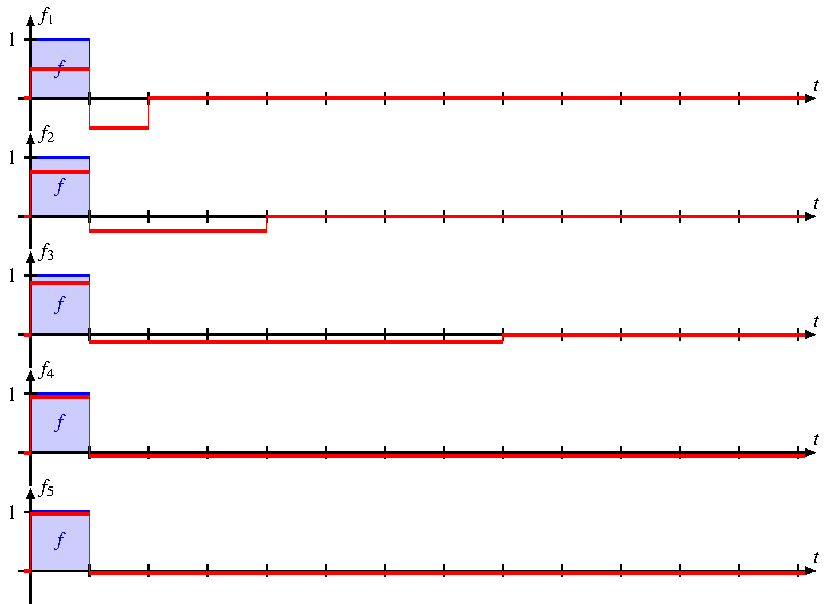
\includegraphics{chapters/3-haar/images/paradox.pdf}
\caption{Approximationsfolge $f_n$, die die Funktion ${\color{blue}\varphi}$
in $L^2(\mathbb R)$ approximiert, aber nicht in $L^1(\mathbb R)$.
\label{haar:fig:paradox}}
\end{figure}

Die Auflösung dieses Paradoxons besteht darin, dass die Funktionen
$f_n$ zwar im $L^2$-Sinn gegen $f$ konvergieren, aber nicht im Sinne von $L^1$.
Dies kann allgemein gezeigt werden, doch ein Beispiel soll dafür genügen.
Die Funktion, die approximiert werden soll, sei die Indikatorfunktion
\[
f(x) = \chi_{[0,1)}(x).
\]
Die Funktion ist das Vaterwavelet.
Die zugehörige Folge $f_n$ ist in Abbildung~\ref{haar:fig:paradox}
dargestellt.
Nach Konstruktion der Haar-Wavelets sind die höherfrequenten Wavelets
darauf orthogonal, daher verschwinden die Skalarprodukte
$\langle \psi_{jk},f\rangle=0$ für $j\ge 0$.
Nur die Funktion $\psi_{j0}$ mit $j<0$ tragen daher etwas dazu bei.
Es ist
\[
\langle \psi_{j0},f\rangle
=
\int_0^1 \psi_{j0}(x)\,dx
=
2^{j/2}.
\]
Daraus kann man jetzt die Approximation für $f$ aufschreiben:
\[
f(x)
=
\sum_{j=-\infty}^{-1} \langle \psi_{j0},f\rangle \psi_{j0}(x)
\psi_{j0}(x).
\]
Es ist klar, dass die Summe $0$ ist für $x<0$.
Wir haben zu überprüfen, dass für $x\in[0,1)$ die Summe gegen $1$ 
korrigiert. 
Für $x>1$ dagegen müsste die Summe gegen $0$ konvergieren.

Wir betrachten erst den Fall $0\le x < 1$.
In diesem Fall ist $\psi_{j0}(x)>0$ für alle Werte von $j\le 0$.
Die Summe ist
\begin{align*}
\sum_{j=-\infty}^{-1} 2^{j/2} \psi_{j0}(x)
&=
\sum_{j=-\infty}^{-1} 2^{j/2} 2^{j/2}
=
\sum_{j=1}^\infty 2^j = 1.
\end{align*}
Im Intervall $[0,1)$ hat die Summe den erwarteten Wert.

Sei jetzt $x>1$.
In diesem Fall kann nicht mehr geschlossen werden, dass alle Terme den
gleichen Wert haben.
Vielmehr gibt es ein $l<0$ derart, dass $x < 2^{-l}$.
Dies bedeutet, dass
\[
\psi_{j0}(x)
=
\begin{cases}
0&\qquad j>l\\
2^{j/2}&\qquad j = l
\\
-2^{j/2}&\qquad j < l.
\end{cases}
\]
Damit kann die Summe ausgewertet werden:
\begin{align*}
\sum_{j=-\infty}^{-1} 2^{j/2} \psi_{j0}(x)
&=
\sum_{j=-\infty}^{l-1} 2^{j/2} 2^{j/2}
-
\sum_{j=l}^{l} 2^{j/2} 2^{j/2}
=
\sum_{j=-\infty}^{l-1} 2^j
-
2^l
=
2^l
-
2^l
=
0.
\end{align*}
Wir schliessen daraus, dass 
\[
\lim_{n\to\infty} f_n(x) = f(x)
\]
für jeden Punkt $x\in\mathbb R$, die Approximationen konvergieren also
punktweise gegen $f(x)$, nicht nur im Sinne von $L^2$.

Um das Paradoxon aufzulösen, müssen wir jetzt die Konvergenz der
Funktionenfolge $f_n$ im $L^1$ Sinne untersuchen.
Dazu müssen wir das Integral
\begin{align}
\| f_n-f\|_1
&=
\int_{\mathbb R} |f_n(x) - f(x)| \,dx
=
\int_0^1 |f_n(x) - f(x)|\,dx
+
\sum_{l=-\infty}^{-1}
\int_{2^{-l-1}}^{2^{-l}} |f_n(x)-f(x)|\,dx
\label{haar:paradox-summe}
\end{align}
berechnen.
Im ersten Integral ist $f(x)=1$, ausserdem ist $f_n(x)$ in diesem Intervall
konstant, so dass dieser Teil zu
\begin{align*}
\int_0^1 |f_n(x) - f(x)|\,dx
&=
\sum_{j=-n}^{-1} 2^{j/2} 2^{j/2} - 1
=
\sum_{j=1}^{n} 2^{-j} - 1
=
\frac12
\frac{1-2^{-n}}{1-2^{-1}}-1
=
2^{-n}
\end{align*}
wird.

Die zweite Summe kann vereinfacht werden, weil die Funktion $f(x)$ in all
diesen Teilintervallen verschwindet.
Ausserdem ist die Funktion $f_n$ in jedem dieser Intervalle konstant
und der Term $j=l$ in der Summe ist negativ.
Die Summe ist dann
\begin{align*}
\int_{2^{-l-1}}^{2^{-l}} |f_n(x)-f(x)|\,dx
&=
\int_{2^{-l-1}}^{2^{-l}} |f_n(x)|\,dx
=
2^{-l-1} 
\biggl|
-2^{l}
+
\sum_{j=-n}^{l-1}  2^{j}
\biggr|
=
2^{-1} 
\biggl|
-1
+
\sum_{j=-n-l}^{-1}  2^{j}
\biggr|
=
2^{-n-l-1}.
\end{align*}

Die Summe auf der rechten Seite von~\eqref{haar:paradox-summe} ist
endlich, da die Funktion $f_n(x)$ verschwindet für $x>2^n$, die Summe
ist also nur bis $l=-n$ zu erstrecken.

Die Summe all dieser Terme ist jetzt die $L^1$-Norm
\begin{align*}
\|f_n - f\|
&=
2^{-n} + \sum_{l=-n}^{-1} 2^{-n-l-1}
=
2^{-n} + 2^{-n-1} + \dots 2^{-1}
=
1- 2^{-n}.
\end{align*}
Die $L^1$-Norm ist also beliebig nahe bei $1$, die Summe kann daher
nicht im Sinne der $L^1$-Norm konvergieren.

